\chapter{Entropy, Equilibrium, and the Maximum-Entropy Problem}

We begin this lecture by rebuilding the statistical-mechanical vocabulary from the ground up: a discrete set of states, a probability distribution over those states, the associated energies, and the entropy functional. From there the lecture moves quickly. A family of equilibrium distributions is drawn and interpreted, the thermodynamic laws are recast in probabilistic language, the direction of heat flow is derived from the definition of temperature, and finally the whole subject is turned into a concrete mathematical problem: find the probability distribution that maximizes entropy subject to fixed total probability and fixed average energy.

\paragraph{Credit.} These notes follow Leonard Susskind's lecture, with lecture curation by LazyingArt LLC and Video2Book.

\section{Entropy, Probability, and Average Energy}

Take a system whose microstates are labeled by an index \(i\). The lecture begins by assuming that, for the moment, the states are discrete so that they can be counted. Each state carries a probability \(P(i)\), and each state also has an energy \(E(i)\). The first two ingredients are then the normalization of probability and the definition of average energy:
\begin{align}
\sum_i P(i) &= 1, \\
\sum_i P(i)E(i) &= \langle E\rangle .
\end{align}
The entropy associated with this probability distribution is
\begin{equation}
S=-\sum_i P(i)\log P(i).
\end{equation}
The point is worth pausing over. Entropy here is not introduced as a mechanical quantity like energy or momentum. It is attached to a probability distribution, and therefore to our incomplete knowledge of which state the system actually occupies.

The minus sign makes the entropy positive. Since \(0<P(i)\le 1\), we have \(\log P(i)\le 0\), and so each term \(-P(i)\log P(i)\) is nonnegative. The lecture emphasizes this because at first sight the formula looks negative even though it is not.

\begin{figure}[htbp]
\centering

\includegraphics[width=0.88\textwidth]{lecture_03_figure_02.png}
\caption{The opening board layout: entropy, the two constraints, and a family of probability distributions drawn against energy.}
\end{figure}

The board is already telling us more than the formulas alone. It places the entropy functional beside the two constraints, and below them it draws a whole family of distributions rather than a single one. That is the next step of the lecture.

\section{Equilibrium as a Family of Distributions}

The lecture does not present equilibrium as one isolated probability distribution. Instead, it begins with a one-parameter family of distributions, parameterized by average energy. They are drawn schematically as distributions over states arranged by energy. As the distribution broadens and shifts toward larger \(E\), the average energy increases.

A special case sits at one end of the family: the ground state. All the probability is concentrated on the state of minimum energy. In that case the entropy is zero, because there is no uncertainty left about which state the system occupies.

What matters for the later thermodynamic discussion is the qualitative picture: as the distribution broadens, more states become relevant, the average energy rises, and the entropy rises with it. The lecture takes this as the characteristic behavior of the thermal-equilibrium family.

\begin{figure}[htbp]
\centering
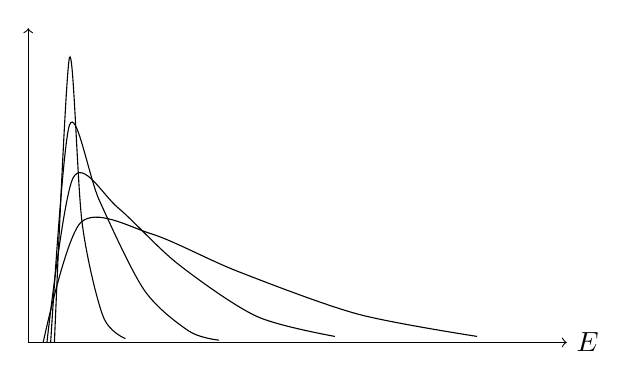
\begin{tikzpicture}[scale=0.95]
\draw[->] (0,0) -- (7.2,0) node[right] {$E$};
\draw[->] (0,0) -- (0,4.2);
\draw[smooth] plot coordinates {(0.35,0) (0.55,3.8) (0.72,1.6) (1.00,0.35) (1.30,0.05)};
\draw[smooth] plot coordinates {(0.30,0) (0.55,2.9) (0.95,1.9) (1.55,0.70) (2.15,0.15) (2.55,0.03)};
\draw[smooth] plot coordinates {(0.25,0) (0.60,2.2) (1.20,1.8) (2.00,1.05) (3.05,0.35) (4.10,0.08)};
\draw[smooth] plot coordinates {(0.20,0) (0.70,1.6) (1.65,1.45) (2.80,0.95) (4.40,0.38) (6.00,0.08)};
\end{tikzpicture}
\caption{A clean schematic version of the family of equilibrium distributions. The picture is qualitative: broader distributions correspond to larger average energy and larger entropy.}
\end{figure}

This is not yet a theorem. It is a physically motivated picture of the equilibrium distributions that will matter in statistical mechanics.

\subsection{Question \& Answer}

A natural objection appears immediately: could one not invent a distribution that moves to the right but narrows instead of broadening? Yes, one could. The lecture explicitly says so. Nothing in pure probability prevents such a family. The important restriction is that the thermal-equilibrium distributions we care about are not of that type. For those equilibrium distributions, the lecture assumes that entropy is a monotonically increasing function of average energy.

\section{The Thermodynamic Laws in Statistical Language}

With the family of distributions in place, the lecture turns to the laws of thermodynamics and reads them statistically.

The first law is simply energy conservation. The second law, in this probabilistic language, says that entropy increases. But what does that mean? The lecture answers: when a system is out of equilibrium and then relaxes toward equilibrium, its probability distribution generally broadens. Under coarse-graining we lose track of microscopic details, not gain them. A narrowing distribution would mean that we had learned more and more about a huge complicated system without having measured it. That is not the typical direction of evolution.

The zeroth law is then not treated as a detached axiom. Instead, it is illuminated by the previously introduced notion of temperature. There exists a temperature function such that energy flows from higher temperature to lower temperature, and when all parts of the system share the same temperature, the flow stops.

To connect these statements, the lecture considers two subsystems \(A\) and \(B\) that can exchange energy. Assume for the moment that \(T_B>T_A\). The total system is closed, so
\begin{equation}
dE_A+dE_B=0.
\end{equation}
The second law says that the total entropy does not decrease:
\begin{equation}
dS_A+dS_B\ge 0.
\end{equation}
Now use the definition of temperature in the form
\begin{equation}
dE=T\,dS.
\end{equation}
Applied separately to the two subsystems,
\begin{equation}
dE_A=T_A\,dS_A,
\qquad
dE_B=T_B\,dS_B.
\end{equation}
Substituting into energy conservation gives
\begin{equation}
T_A\,dS_A+T_B\,dS_B=0.
\end{equation}
Solving for \(dS_B\),
\begin{equation}
dS_B=-\frac{T_A}{T_B}\,dS_A.
\end{equation}
Insert this into the entropy inequality:
\begin{align}
dS_A+dS_B &\ge 0, \\
dS_A-\frac{T_A}{T_B}dS_A &\ge 0, \\
\left(1-\frac{T_A}{T_B}\right)dS_A &\ge 0.
\end{align}
For positive temperatures, multiply through by \(T_B\):
\begin{equation}
(T_B-T_A)dS_A \ge 0.
\end{equation}
But we assumed \(T_B>T_A\), so the factor \(T_B-T_A\) is positive. Therefore
\begin{equation}
dS_A>0.
\end{equation}
Multiplying by \(T_A\) gives
\begin{equation}
dE_A=T_A\,dS_A>0.
\end{equation}
Thus subsystem \(A\) gains energy, subsystem \(B\) loses it, and energy flows from the hotter subsystem to the colder one. In the lecture, ``heat'' here simply means this energy transfer.

The conclusion is exactly the zeroth-law statement we wanted: temperature determines the direction of heat flow, and equilibrium is the condition in which the temperatures become equal and the flow stops.

\subsection{Question \& Answer}

A student asks whether this argument assumes that \(A\) and \(B\) are each internally in equilibrium. The answer is yes. The derivation uses a temperature \(T_A\) and a temperature \(T_B\), and that already assumes that each subsystem has settled enough internally for such a temperature to make sense. If one of the subsystems is not internally equilibrated, the remedy is not to discard the argument but to subdivide further and apply the same reasoning to smaller pieces.

\section{What a State Means}

At this point the lecture pauses over another foundational question: what is a state?

The answer is direct. A state means as much as can possibly be known about the system by an infinitely powerful observer, subject to the actual laws of physics. For a classical gas one naturally thinks of the positions and momenta of all the molecules, although in classical language those variables are continuous. In quantum mechanics, for a finite box, the state counting becomes discrete. The lecture does not force a heavy formalism here. It simply says that, in the classical limit, sums are replaced by integrals.

That clarification matters. The entropy formula was written as a sum because the lecture is counting discrete states. But the conceptual content is broader: the entropy measures the uncertainty associated with a probability distribution over the most refined states that the theory allows us to discuss.

\subsection{Question \& Answer}

Should one literally think of a state of a gas as the complete microscopic specification of all particle positions and momenta? As a first classical picture, yes. But the lecture immediately qualifies this: quantum mechanics limits what can be known simultaneously, and in the quantum treatment the state counting becomes discrete. The useful invariant idea is not ``position and momentum'' by itself, but ``the finest state-description allowed by the laws of physics.''

\section{Heat Baths, Replicas, and Probability as Fraction}

The next question is the real open problem of the lecture: once equilibrium has been reached, what is the actual probability distribution over microstates?

To make the question concrete, the lecture introduces a heat bath. Instead of treating our system as perfectly isolated, we imagine it in contact with a very large outside world that can exchange energy with it. Because the reservoir is so large, a small transfer of energy barely changes its temperature.

A particularly convenient model of the heat bath is then introduced: replace the large reservoir by a large number \(N\) of identical copies of the subsystem. One copy is the system we care about; the others play the role of the bath. Each copy occupies some state \(i\), and we define the occupation number \(n_i\) to be the number of copies in state \(i\).

The board at this point makes the transition from counting to probability explicit.

\begin{figure}[htbp]
\centering

\includegraphics[width=0.82\textwidth]{lecture_03_figure_03.png}
\caption{Probability written as occupation fraction: \(P(i)=n_i/N\).}
\end{figure}

This is the key identification:
\begin{equation}
P(i)=\frac{n_i}{N}.
\end{equation}
Probability is the fraction of the replicas that occupy the \(i\)-th state.

There are two constraints. First, the total number of replicas is fixed:
\begin{equation}
\sum_i n_i = N.
\end{equation}
Second, the total energy is fixed. If \(e_i\) denotes the energy of the \(i\)-th state, and \(E\) denotes the average energy per subsystem, then
\begin{equation}
\sum_i n_i e_i = N E.
\end{equation}
Using \(n_i=NP_i\), these become the familiar probability constraints:
\begin{align}
\sum_i P_i &= 1, \\
\sum_i P_i e_i &= E.
\end{align}
At this point the lecture has converted a thermodynamic equilibrium problem into a problem about occupation numbers and probabilities.

\section{Multiplicity, Stirling's Approximation, and Entropy}

Now comes the combinatorial part. Fix a set of occupation numbers \(\{n_i\}\). How many ways are there to distribute the \(N\) replicas among the states so that these occupation numbers result? The answer is
\begin{equation}
C=\frac{N!}{\prod_i n_i!}.
\end{equation}
This \(C\) is the multiplicity: the number of arrangements consistent with the chosen occupation numbers. Unoccupied states cause no trouble because
\begin{equation}
0!=1.
\end{equation}

The lecture checks the formula against simple examples, but the real point is that the most probable occupation pattern is the one with the largest multiplicity. So we must maximize \(C\), subject to the two constraints above.

For large \(N\), the lecture introduces the simplified Stirling approximation
\begin{equation}
N!\approx N^N e^{-N}.
\end{equation}
A short derivation is given by taking logarithms:
\begin{equation}
\log N! = \sum_{x=1}^N \log x \approx \int_1^N \log x\,dx.
\end{equation}
Since
\begin{equation}
\int \log x\,dx = x\log x-x,
\end{equation}
we obtain
\begin{equation}
\log N! \approx N\log N-N,
\end{equation}
and exponentiating gives the stated approximation. The lecture notes that this omits subleading corrections, including the familiar \(\sqrt{2\pi N}\) factor, but those are not important for the present argument.

Apply the same approximation to the numerator and denominator of \(C\):
\begin{equation}
C
\approx
\frac{N^N e^{-N}}{\prod_i n_i^{\,n_i} e^{-n_i}}.
\end{equation}
Because \(\sum_i n_i=N\), the exponential factors cancel, and we are left with
\begin{equation}
C\approx \frac{N^N}{\prod_i n_i^{\,n_i}}.
\end{equation}
Take the logarithm:
\begin{equation}
\log C = N\log N-\sum_i n_i\log n_i.
\end{equation}
Now substitute \(n_i=NP_i\). Then
\begin{equation}
\log n_i = \log(NP_i)=\log N+\log P_i,
\end{equation}
so
\begin{align}
\log C
&= N\log N-\sum_i NP_i\bigl(\log N+\log P_i\bigr) \\
&= N\log N - N\log N\sum_i P_i - N\sum_i P_i\log P_i.
\end{align}
Since \(\sum_i P_i=1\), the first two terms cancel:
\begin{equation}
\log C = -N\sum_i P_i\log P_i = NS.
\end{equation}
This is the conceptual payoff of the lecture. Maximizing multiplicity is the same as maximizing entropy. Therefore the equilibrium probability distribution is the one that maximizes
\begin{equation}
S(P_i)=-\sum_i P_i\log P_i
\end{equation}
subject to
\begin{equation}
\sum_i P_i=1,
\qquad
\sum_i P_iE_i=E.
\end{equation}

\subsection{Question \& Answer}

A student asks whether, by symmetry, all the occupation numbers should simply be equal. The answer is: only if we forget the energy constraint. Without constraints, a uniform distribution would indeed be the natural extremum. But the states have different energies, and the condition of fixed average energy breaks that symmetry. The correct problem is not to maximize entropy freely, but to maximize it subject to both normalization and fixed average energy.

\section{Lagrange Multipliers and the Mathematical Problem Left for Next Time}

The lecture does not yet solve the maximum-entropy problem. Instead it introduces the necessary tool: Lagrange multipliers.

The geometric picture comes first. Suppose we want to maximize a function \(F\) subject to a constraint
\begin{equation}
G(x_1,x_2,\dots)=0.
\end{equation}
On a contour plot of \(F\), the constrained extremum occurs where a level curve of \(F\) is tangent to the constraint curve \(G=0\).

\begin{figure}[htbp]
\centering
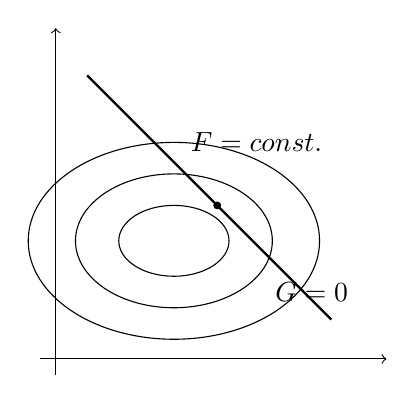
\begin{tikzpicture}[scale=1.0]
\draw[->] (-0.2,0) -- (4.2,0);
\draw[->] (0,-0.2) -- (0,4.2);
\draw (1.5,1.5) ellipse (0.7 and 0.45);
\draw (1.5,1.5) ellipse (1.25 and 0.85);
\draw (1.5,1.5) ellipse (1.85 and 1.25);
\draw[thick] (0.4,3.6) -- (3.5,0.5);
\fill (2.05,1.95) circle (0.05);
\node at (3.25,0.85) {$G=0$};
\node at (2.55,2.75) {$F=\text{const.}$};
\end{tikzpicture}
\caption{Interpretive sketch of constrained optimization: the extremum of \(F\) along \(G=0\) occurs at tangency.}
\end{figure}

The analytic trick is then stated. Instead of extremizing \(F\) under the condition \(G=0\), define a new function
\begin{equation}
F' = F+\lambda G,
\end{equation}
where \(\lambda\) is the Lagrange multiplier. One extremizes \(F'\) as if \(\lambda\) were an additional variable, and then imposes the constraint \(G=0\) at the end.

The worked example is
\begin{equation}
F=\frac{x^2+y^2}{2},
\qquad
G=x+y-1.
\end{equation}
Then
\begin{equation}
F'=\frac{x^2+y^2}{2}+\lambda(x+y-1).
\end{equation}
The stationarity equations are
\begin{align}
\frac{\partial F'}{\partial x} &= x+\lambda = 0, \\
\frac{\partial F'}{\partial y} &= y+\lambda = 0.
\end{align}
Thus
\begin{equation}
x=y=-\lambda.
\end{equation}
Now impose the constraint:
\begin{equation}
x+y=1.
\end{equation}
Therefore
\begin{equation}
-2\lambda=1,
\qquad
\lambda=-\frac12,
\end{equation}
and hence
\begin{equation}
x=y=\frac12.
\end{equation}
This is the minimum of \(F\) on the line \(x+y=1\).

The lecture then states the general rule: for several constraints \(G_1=0\), \(G_2=0\), and so on, add one multiplier for each constraint:
\begin{equation}
F' = F+\lambda_1 G_1+\lambda_2 G_2+\cdots.
\end{equation}
One then solves the stationarity equations together with the constraints themselves.

This is exactly the machinery needed for statistical mechanics. The real problem, left for the next lecture, is now completely clear:
\begin{equation}
\text{maximize } S(P_i)=-\sum_i P_i\log P_i
\end{equation}
subject to
\begin{equation}
\sum_i P_i=1,
\qquad
\sum_i P_iE_i=E.
\end{equation}
The unknowns are the probabilities \(P_i\). Once those are found, the equilibrium distribution is found. The lecture even signals the next payoff in advance: temperature itself will emerge as a Lagrange multiplier.

\section{Summary}

The lecture begins with the entropy of a probability distribution and keeps that definition in view throughout. Equilibrium is first pictured as a family of distributions whose entropy rises with average energy. The thermodynamic laws are then reinterpreted probabilistically, and from \(dE=T\,dS\) together with energy conservation and entropy increase we derive the direction of heat flow. After that the problem is reformulated through replicas and occupation numbers, the multiplicity is counted, and Stirling's approximation turns \(\log C\) into \(NS\). The final result is therefore not yet the explicit equilibrium distribution, but something sharper in a way: the whole subject has been reduced to one mathematical instruction, namely to maximize entropy subject to the appropriate constraints.